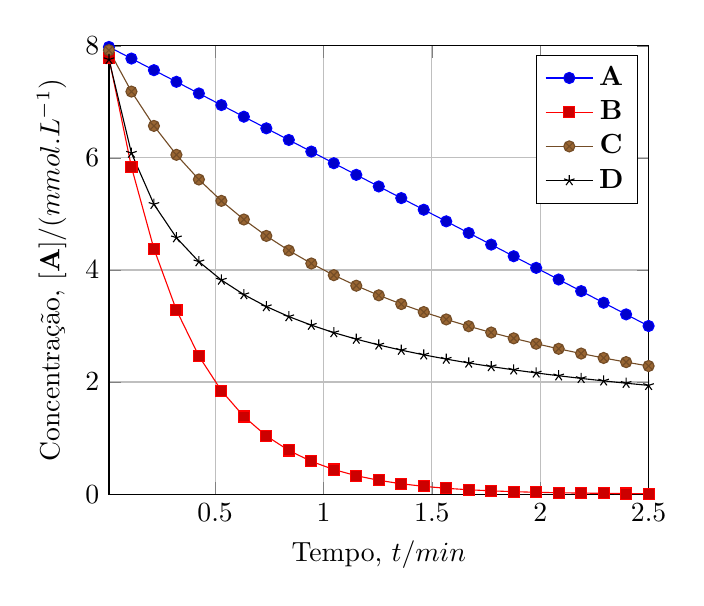
\begin{tikzpicture}
    \begin{axis}
        [
            xlabel = {Tempo, $t/\unit{min}$},
            ylabel = {Concentração, $[\ce{\textbf{A}}]/(\unit{mmol.L^{-1}})$},
            xmin = 0.01, xmax = 2.5,
            ymin=0, ymax = 8,
            domain = 0.01:2.5,
            grid = major,
        ]
    \addplot
        {
            8-2*x
        };
    \addplot
        {
            8*e^(-2.7726*x)
        };
    \addplot
        {
            (1/8 + x/8)^(-1)
        };
    \addplot
        {
            (1/8^2 + 0.1*x)^(-1/2)
        };
    \legend{\textbf{A}, \textbf{B}, \textbf{C}, \textbf{D}}
    \end{axis}
\end{tikzpicture}